\newpage
\section{DIAGRAMAS DO PROJETO}

\subsection{Diagrama de Classes}
O diagrama de classes foi construído com base nos requisitos funcionais e não funcionais estipulados, e representa as regras de negócio da aplicação.
O diagrama pode ser visualizado na Figura \ref{fig:diagramaClasses}.

\begin{figure}[h]
    \centering
    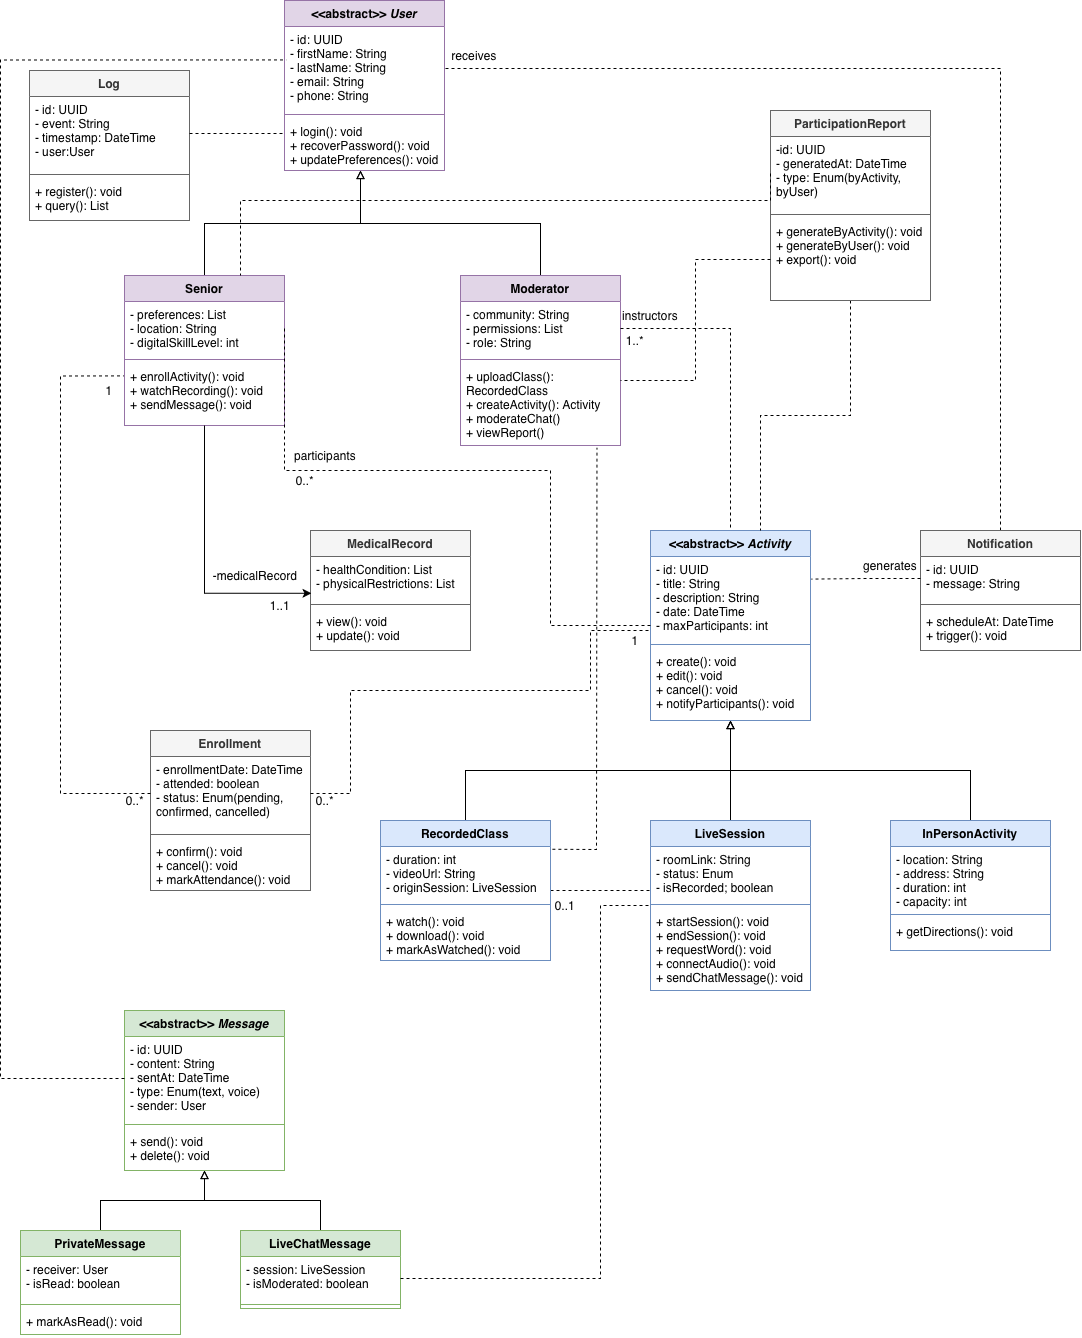
\includegraphics[width=0.8\linewidth]{images/classes_senior.png}
    \caption{Diagrama de Classes}
    \label{fig:diagramaClasses}
\end{figure}

\subsection{Diagrama de Sequência}
O diagrama de sequencia construido demonstra o funcionamento das aulas gravadas dentro da plataforma, e pode ser visualizado na Figura \ref{fig:diagramaSequencia}.

\begin{figure}[h]
    \centering
    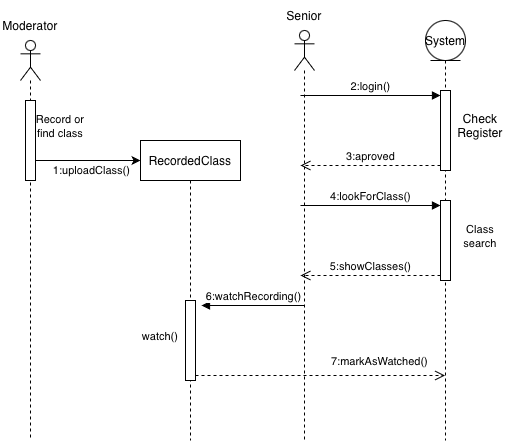
\includegraphics[width=0.8\linewidth]{images/sequencia.png}
    \caption{Diagrama de Sequência}
    \label{fig:diagramaSequencia}
\end{figure}

\subsection{Diagrama de Atividades}
O diagrama de sequencia construido demonstra o funcionamento das reuniões ao vivo dentro da plataforma, assim cobrindo as principais funcionalidades necessárias para a aplicação.
Este diagrama pode ser visualizado na Figura \ref{fig:diagramaAtividades}.

\begin{figure}[h]
    \centering
    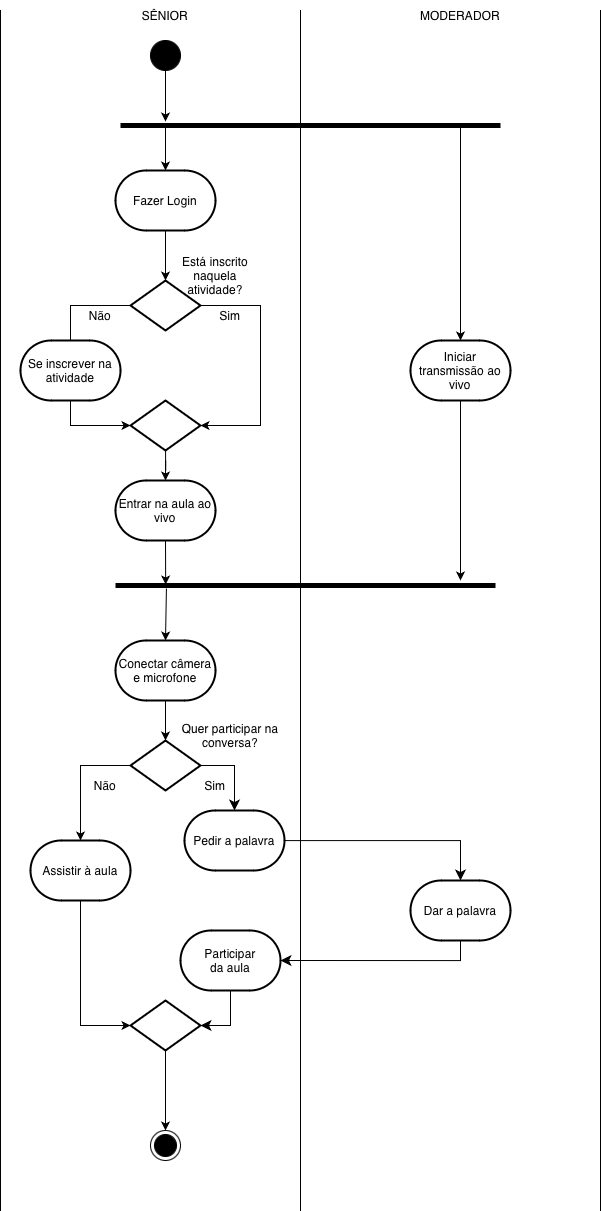
\includegraphics[width=0.8\linewidth]{images/atividades.png}
    \caption{Diagrama de Atividades}
    \label{fig:diagramaAtividades}
\end{figure}

\subsection{Diagrama de Pacotes}
O diagrama de pacotes mostra a separação das classes do modelo de negócio em pacotes, além dos pacotes das outras camadas que serão necessárias para implementar a plataforma funcionalidades
Isso pode ser visualizado na Figura \ref{fig:diagramaPacotes}.

\begin{figure}[h]
    \centering
    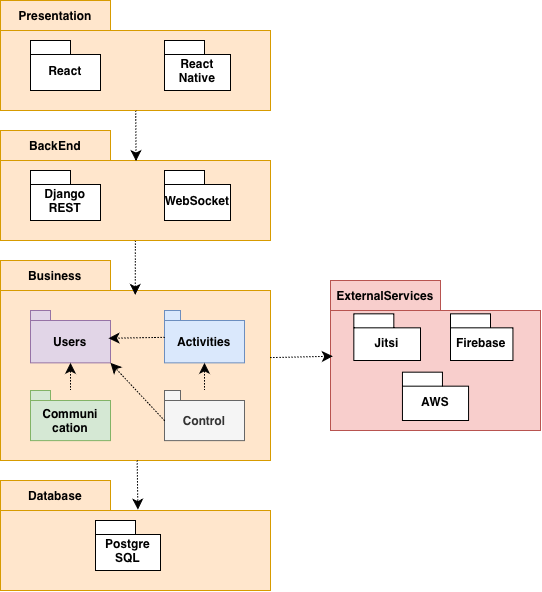
\includegraphics[width=0.8\linewidth]{images/pacotes.png}
    \caption{Diagrama de Atividades}
    \label{fig:diagramaPacotes}
\end{figure}